\chapter{State-of-the-Art}
\section{Overview}
The role of Machine Learning has continuously growth in the past few years and a lot of efforts has been done for developing good software APIs in order to address different needs and domains. \newline In principle, all the machine learning algorithms can be run on the CPU, which already runs the OS and other Application Softwares, this leads to a lot of overheads, especially in terms memory accesses which are expensive in terms of energy and latency. \\\\
Analyzing machine learning algorithms it comes evident that they massively do the same operations and access to data with some kind of patterns. Thus, with the outcome of the new paradigm for the GPU, the General Purpose GPU programming it comes in handy that implementing those algorithms on a GPU, which matches the Machine Learning algorithms requirements regarding the massive operations and the reuse of data, has given a lot of advantages in terms of latency and energy efficiency. However, the capability of GPU of running machine learning algorithms has been pushed almost at the maximum with the increase of computation demands in modern neural networks, therefore other solutions have been explored, such as the development of specific hardware platform.

\section{GPU}
The Moore's law is reaching the end from the point of view of CPUs. However, it seems that the GPUs can still carry on the Moore's law \cite{5496638}.\newline
For this reason, a lot of improvements especially from the companies have been made for developing more and more GPUs with a lower performance per watts.\\
As already mentioned, with the income of general purpose GPU programming paradigm, more and more machine learning algorithms have been designed for being run on the GPU, gathering the best fruits given by that type of architecture.\\\\
As consequences, companies such as Nvidia have started to develop GPU for boosting machine learning applications performance.
\subsection{Nvidia Ampere A100 Tensor Core GPU}
The Nvidia Ampere A100 Tensor Core GPU has been announcer recently and it is one of the most performant GPU. The newly added Tensor Core Unit allows massive increases in throughput and efficiency.\\It is able to deliver up to 624 TFPLOPS\footnote{floating point operations per second} for training and inference machine learning applications.\\\\

The GPU is composed of multiple GPU processing clusters (GPCs), texture processing clusters (TPCs) and streaming multiprocessors (SMs).

The core of the GPU is the Streaming Multiprocessor, which is built up from the SM of Volta GPU and Turing GPU.
\begin{figure}[!htbp]
\centering
\captionsetup{justification=centering}
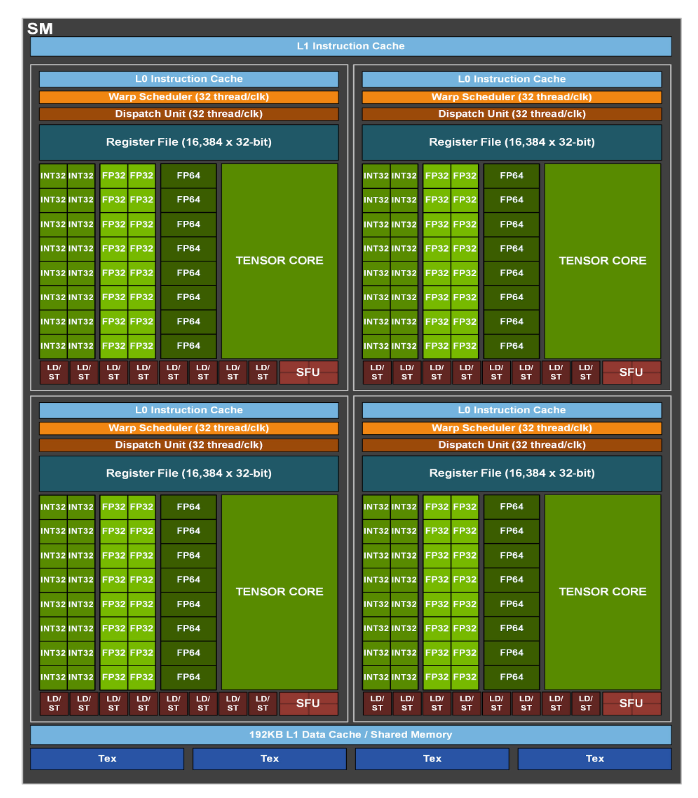
\includegraphics[scale=0.8]{./figure/volta_sm_arch.PNG}
\caption{Streaming Multiprocessor Architecture \cite{paper:41}}
\label{fig:voltasmarch}
\end{figure}


Composed of integer, FP32, FP64 units and the Tensor Core Units designed specifically for deep learning.It introduces also new data types in the tensor core for the computation,binary , integer 8 and 4 bits, floating point 64, 32,16 and bfp16 (the throughput of the tensor core computation for fp16 and bfp16 is the same). The Ampere SM can achieve such efficient workload on mixed computation and addressing calculations thanks to an independent parallel integer and floating-point data paths, sparsity execution feature in Tensor Core. \\\\

Matrix-Matrix multiplication operations are at the core of neural network training and inference, and are used to multiply large matrices of input data and weights in the connected layers of the network. The idea is represented into the Figure \ref{fig:tensorcorevolta} and compered to previous architectures.

\begin{figure}[!htbp]
\centering
\captionsetup{justification=centering}
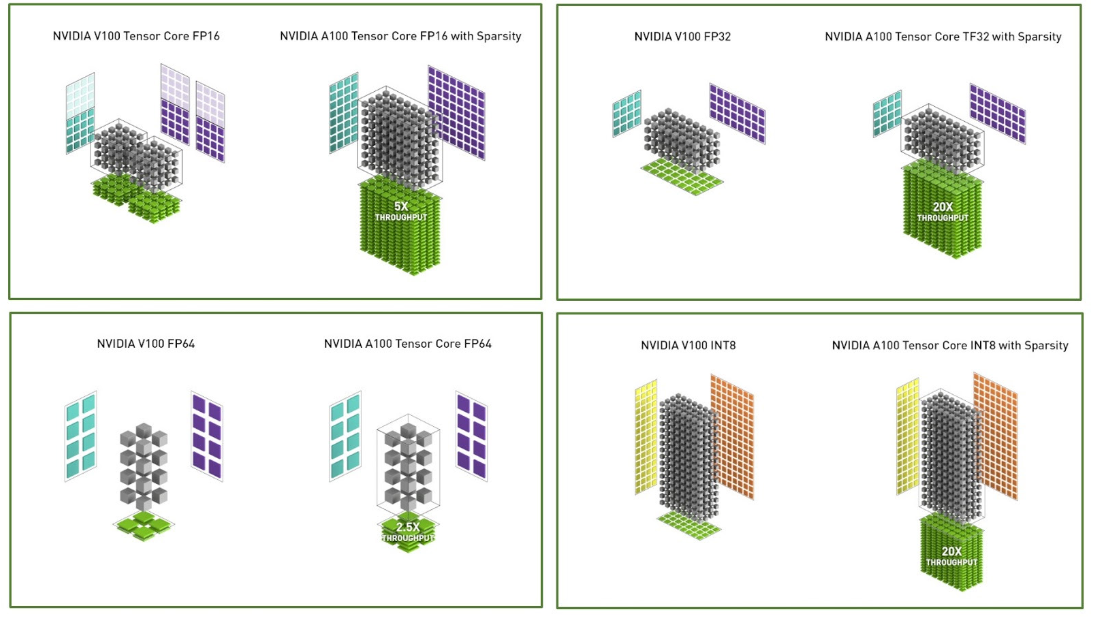
\includegraphics[scale=0.6]{./figure/tensor_core.PNG}
\caption{Matrix Multiplication in Tensor Core\cite{paper:41}}
\label{fig:tensorcorevolta}
\end{figure}

The Ampere A100 GPU contains 108 Streaming multipressor, and 432 third generation Tensor Core.
According to Figure \ref{fig:mixprec} the Tensor Core Units are able to compute multiplications on FP16 and accumulate on FP32, leading to a further reduction of latency and energy consumption.
\begin{figure}[!htbp]
\centering
\captionsetup{justification=centering}
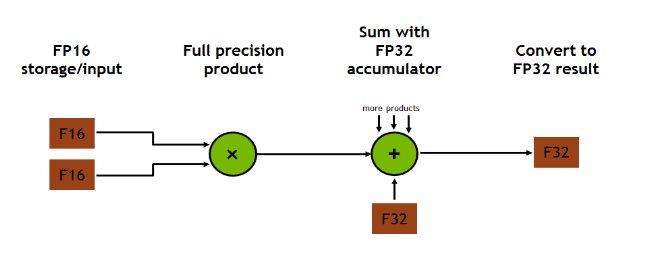
\includegraphics[scale=0.8]{./figure/mix_prec.PNG}
\caption{Mixed Precision Schema of a FMA unit in Tensor Core Unit\cite{paper:41}}
\label{fig:mixprec}
\end{figure}

\newpage
The deep learning frameworks and the CUDA Toolkit include libraries that have been custom-tuned to provide high multi-GPU performance for each one of the following deep learning frameworks in the Figure \ref{fig:swtesla}.

\begin{figure}[!htbp]
\centering
\captionsetup{justification=centering}
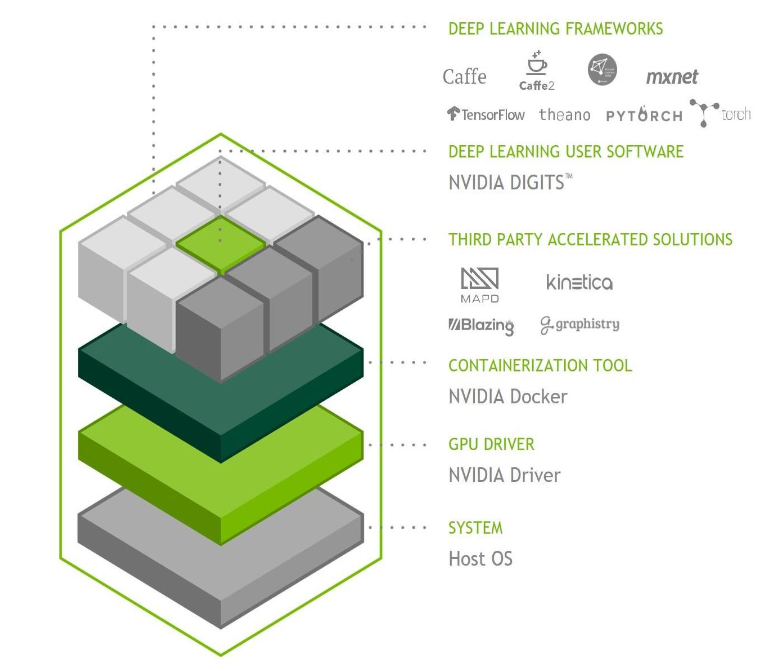
\includegraphics[scale=0.6]{./figure/sw_stack_tesla.PNG}
\caption{Software stack\cite{paper:41}}
\label{fig:swtesla}
\end{figure}

Combining powerful hardware with software tailored to deep learning, it provides to developers and researchers solutions for high-performance GPU-accelerated deep learning application development, testing, and network training.
\newpage
\section{Domain Specific Hardware Platform}
Instead of developing GPUs also suitable for Machine Learning applications, the companies have designed and deployed special purpose hardware accelerators.
\subsection{NVDLA}
The Nvidia Deep Learning Accelerator is a free open source hardware platform from Nvidia, highly customizable and modular, which allows to design and deploy deep learning inference hardware.

The architecture comes in two configurations:

\begin{figure}[!htbp]
\centering
\captionsetup{justification=centering}
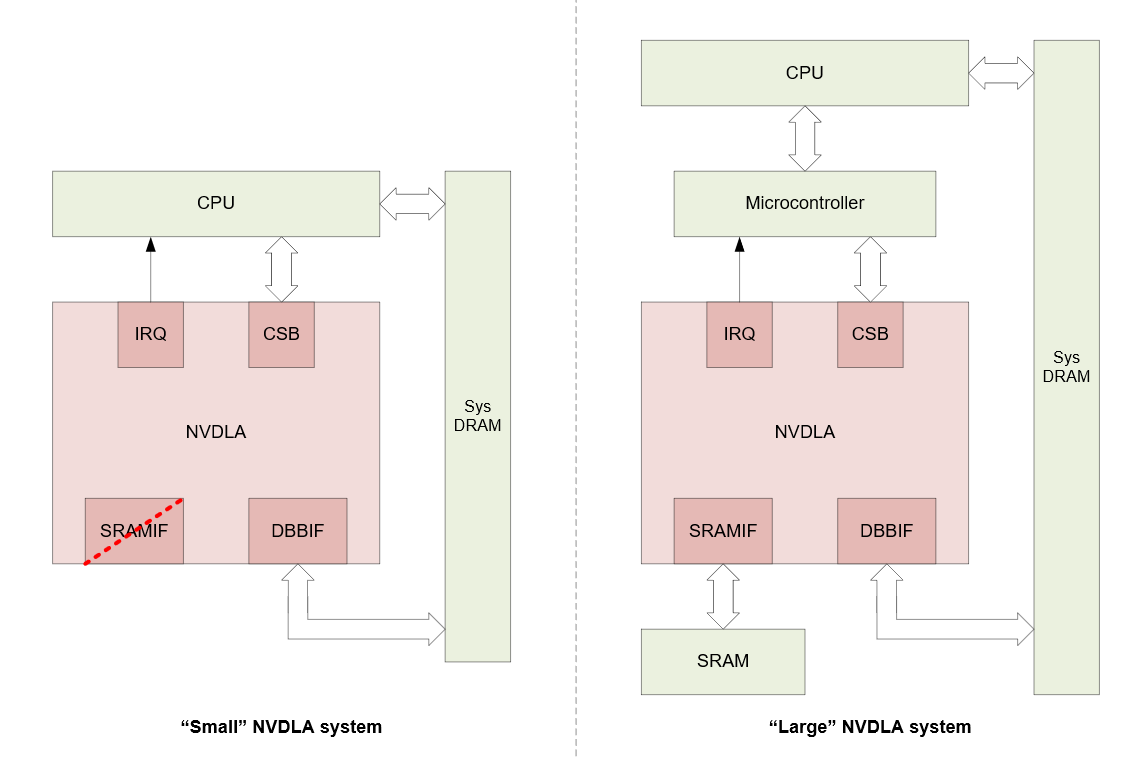
\includegraphics[scale=0.4]{./figure/nvdla_system.PNG}
\caption{Comparsion of two possible NVDLA system\cite{WEBSITE:8}}
\label{fig:nvdlasystem}
\end{figure}
As already mentioned, the aim of the work is to develop a hardware accelerator for machine learning suitable for mobile devices, therefore from now on the NVDLA small system will be considered and analyzed.\\
The internal architecture of the NVDLA small system is:
\begin{figure}[!htbp]
\centering
\captionsetup{justification=centering}
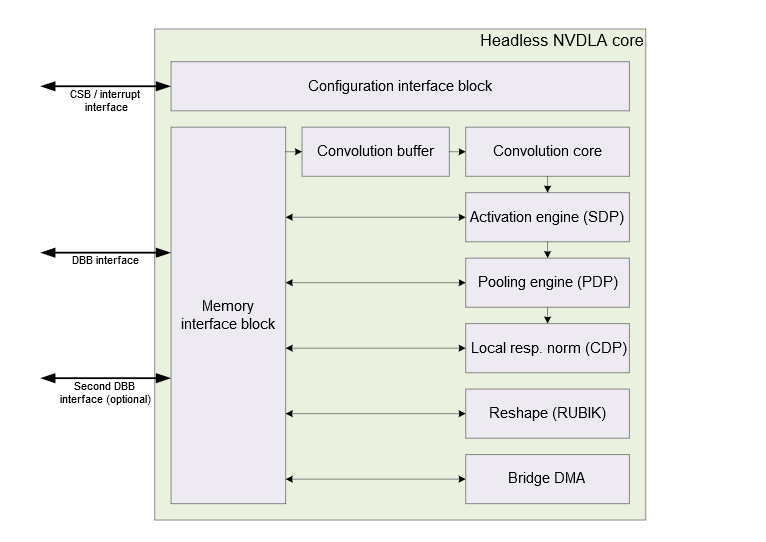
\includegraphics[scale=0.5]{./figure/nvdla_internal.PNG}
\centering\caption{Internal architecture of NVDLA small system, Secondary DBB not considered\cite{WEBSITE:8}}
\label{fig:nvdlaarch}
\end{figure}

According to Figure \ref{fig:nvdlasystem}, for the Small configuration of the accelerator, the processor will be in charge of programming and scheduling the operations on the NVDLA and as consequences handles the start/end of operations and possible interrupts, all of them through the CSB (Configuration Space Bus) interface which is AXI Lite compliant\cite{paper:30}. \newline
The data movement to/from memory are handled by the Internal memory controller though the DBB (Data BackBone) interface, which is AXI \cite{paper:30} compliant.\\

The internal architecture of NVDLA is composed by various engines, each one of them is able to perform specific Machine Learning models:
\begin{itemize}
\item Convolution Core: it comes in pair with the Convolution Buffer, its private memory for the data (inputs and weights). It is used to accelerate the convolution algorithms.
\item Activation engine (Single Data point Operations): it performs post processing operations at the single data element level such as bias addition, Non linear function, PReLU (Parametric Rectified Linear Unit) and format conversion when the software requires different precision for different hardware layers.
\item Pooling engine (Planar Data Operations): it is designed to accomplish pooling layers, i.e. it executes operation along the width and height plane.
\item Local response normalization engine(Cross Channel Data operations): it is designed to address local response normalization layers.
\item Reshape(Data memory and reshape operations): it transforms data mapping format without any data calculation.
\item Bridge DMA: it is in charge of copying data from the Main Memory to the SRAM of the accelerator, only available into the large configuration of the system.
\end{itemize}


Another possible configuration which is worth to mention is the possibility to let the engines work separately on independent task or in a fused fashion where all of them are pipelined, working as a single entity.\\

According to developers the configurability of the cores ranges from arithmetic precision to the theoretical throughput that a single unit can achieve (increasing the number of internal Processing Elements). Moreover, since the engine units are independent from each other, according to the application and the model used they can be safely removed from the design.
\newpage
\subsubsection{ NVDLA Software }
It is also worth to mention that the accelerator comes already with a basic software stack:
\begin{figure}[H]
\centering
\captionsetup{justification=centering}
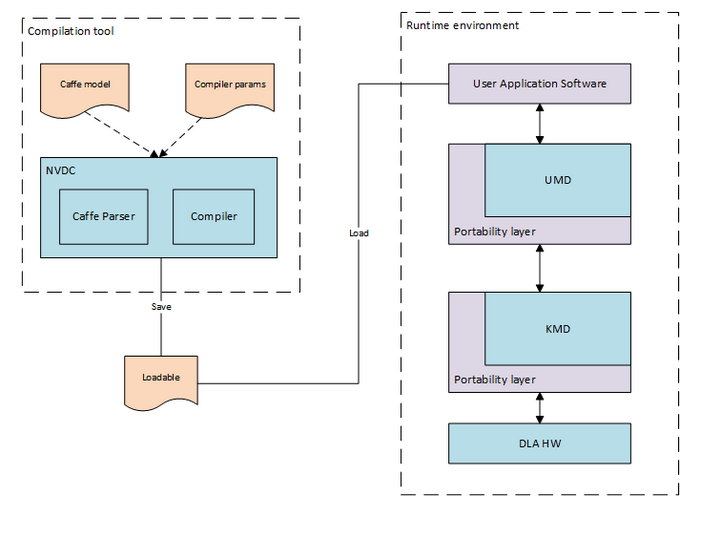
\includegraphics[scale=0.8]{./figure/nvdla_software.PNG}
\caption{NVDLA Software stack\cite{WEBSITE:7}}
\label{fig:nvdlasw}
\end{figure}

Where the Compilation tools are in charge of converting existing pretrained model into a set of hardware layers (for the desired precision) and programming sequences suitable for the NVDLA, the output of this process is a Nvidia Loadable file suitable for the runtime environment.\\
Regarding the runtime environment, it has been designed for a system in which is present an OS. It is composed in two parts: the User Mode Driver (UMD) and the Kernel Mode Driver (KMD).\newline The User Mode Driver loads the loadable file in memory and submits the operation to the KMD, it is also in charge of data movement from/to the accelerator. \newline The KMD is in charge of submit operations to the accelerator through low level functions, schedules the operations and handles the interrupts.\\
Both the KMD and the UMD are wrapped into portability layers which are, respectively, hardware dependent and OS dependent. In principle, for migrating the software to another OS or hw plaftorm it is enough to modify only the portability layers.
\newpage
\subsection{Google TPU}
Google developed its own application-specific integragrated circuit for neural networks, which is tightly integrated with TensorFlow Software.
It includes:
\begin{itemize}
\item Matrix Multiplier Unit (MXU): 65,536 8-bit multiply-and-add units for matrix operations
\item Unified Buffer (UB): 24MB of SRAM that work as registers
\item Activation Unit (AU): Hardwired activation functions
\end{itemize}

In Figure \ref{fig:tpuarch} a general view of TPU architecture is presented.
\begin{figure}[H]
\centering
\captionsetup{justification=centering}
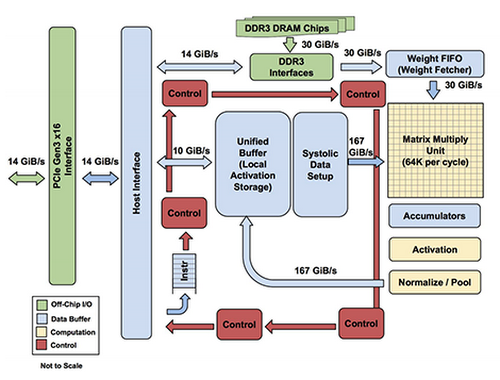
\includegraphics[scale=0.8]{./figure/tpu_arch.PNG}
\caption{Google TPU architecture\cite{paper:40}}
\label{fig:tpuarch}
\end{figure}

Rather than be tightly integrated with a CPU, the TPU is designed to be a coprocessor in which the instruction are sent by the host server rather than fetched.\\\\
The matrix multiplication unit reuses both inputs many times as part of producing the output avoiding the overhead of continuously read data from memory. Only spatial adjacent ALU are connected together, which makes wires shorter and energy-efficient. The ALUs only perform computations in fixed pattern.
\newpage
As far as concern the software stack, the TPU can be programmed for a wide variety of neural network models. To program it, API calls from TensorFlow graph are converted into TPU instructions.
\begin{figure}[H]
\centering
\captionsetup{justification=centering}
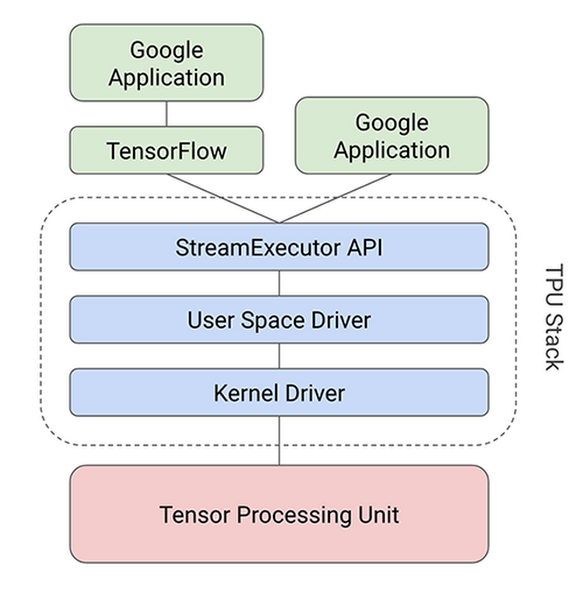
\includegraphics[scale=0.4]{./figure/tpu_sw_stack.PNG}
\caption{Google TPU Software Stack\cite{WEBSITE:9}}
\label{fig:gtpuswstack}
\end{figure}

\subsection{Habana Goya HL-1000}

Habana’s Goya is a processor dedicated to inference workloads. It is designed to deliver superior performance, power efficiency and cost savings for data centers and other emerging applications.\\
It allows the adoption of different deep learning models and is not limited to specific domains. Moreover, the performance requirements and accuracy can be user-defined.\\

In the Figure \ref{fig:goyaarch} a high level view of the Goya architecture can be appreciated.
\begin{figure}[H]
\centering
\captionsetup{justification=centering}
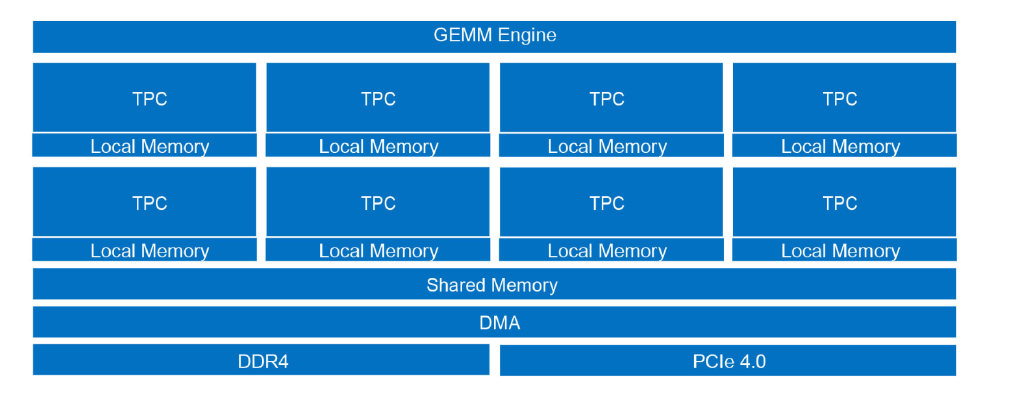
\includegraphics[scale=0.7]{./figure/goya_arch.PNG}
\caption{High level view of Goya architecture\cite{paper:38}}
\label{fig:goyaarch}
\end{figure}

It is based on scalable, fully programmable Tensor Processing Cores, specifically designed for deep learning workloads. \\
It also provides other flexible features such as GEMM operation acceleration, special functions dedicated hardware, tensor addressing, latency hiding capabilities and different data types support in TPC (FP32, INT32, INT16, INT8, UINT32, UINT16, UINT8).\\

Regarding the software stack, it can be interfaced with all deep learning frameworks. However, a model has to be first converted into an internal representation, as it can be seen in Figure \ref{fig:goyaswstack}.
\begin{figure}[H]
\centering
\captionsetup{justification=centering}
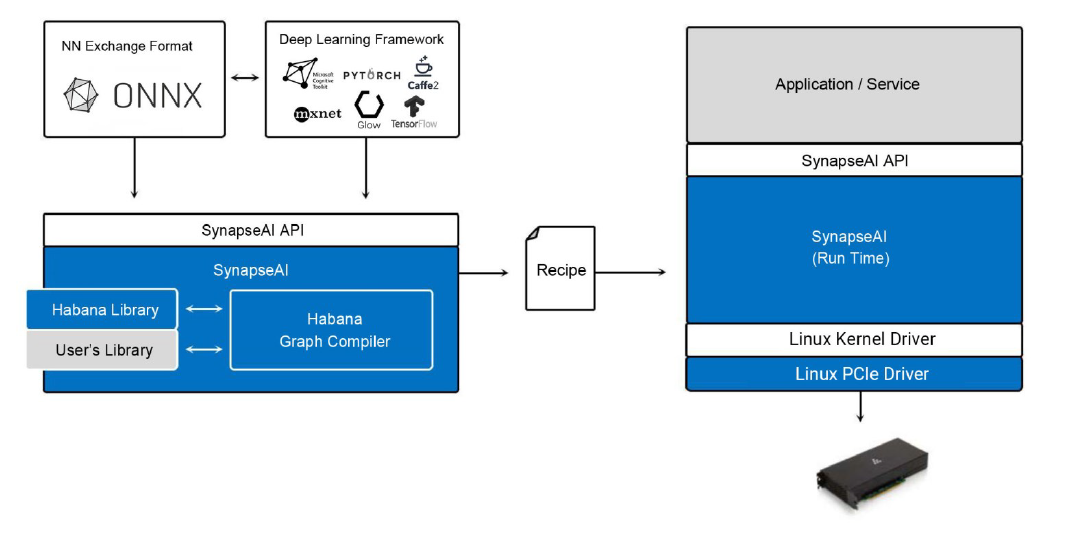
\includegraphics[scale=0.5]{./figure/goya_sw_stack.PNG}
\caption{Habana Goya Software Stack\cite{paper:38}}
\label{fig:goyaswstack}
\end{figure}
It also supports quantization of models trained in floating-point format with near-zero accuracy loss.